\documentclass[10pt,twocolumn,letterpaper]{article}

\usepackage{cvpr}
\usepackage{times}
\usepackage{epsfig}
\usepackage{graphicx}
\usepackage{amsmath}
\usepackage{amssymb}

% Include other packages here, before hyperref.

% If you comment hyperref and then uncomment it, you should delete
% egpaper.aux before re-running latex.  (Or just hit 'q' on the first latex
% run, let it finish, and you should be clear).
\usepackage[breaklinks=true,bookmarks=false]{hyperref}

\cvprfinalcopy % *** Uncomment this line for the final submission

\def\cvprPaperID{****} % *** Enter the CVPR Paper ID here
\def\httilde{\mbox{\tt\raisebox{-.5ex}{\symbol{126}}}}

% Pages are numbered in submission mode, and unnumbered in camera-ready
%\ifcvprfinal\pagestyle{empty}\fi
\setcounter{page}{1}
\begin{document}

%%%%%%%%% TITLE
\title{PCANet and CNN for Image classification}

\author{Yin Zhang\\
Department of Statistics\\
University of Virginia\\
Charlottesville, VA 22903\\
{\tt\small yz4an@virginia.edu}
% For a paper whose authors are all at the same institution,
% omit the following lines up until the closing ``}''.
% Additional authors and addresses can be added with ``\and'',
% just like the second author.
% To save space, use either the email address or home page, not both
\and
Haoran Liu \\
Department of Computer Science \\
University of Virginia\\
Charlottesville, VA 22903  \\
{\tt\small hl4fb@virginia.edu} 
}

\renewcommand{\b}[1] {\boldsymbol{#1}} 
\newcommand{\bb}[1] {\bar{\boldsymbol{#1}}}

\maketitle
%\thispagestyle{empty}

%%%%%%%%% ABSTRACT
\begin{abstract}
In this paper, we reimplement the PCANet proposed by \cite{chan2015pcanet} in torch7. We test the PCANet in CIFAR10 dataset for objection recognition task. We also test two CNNs (one is 2 layers and the other is 3 layers) on this task to compare the performances. We find that the CNNs outperform PCANet in terms of test accuracy and training time. PCANet takes around $8$ hours and gives a test accuracy of $59.06\%$ while the 2 layer CNN results in a test accuracy of $65.02\%$ and the 3 layer CNN results in a test accuracy of $70.82\%$, just taking $0.75$ hour and $1.5$ hour, respectively, on a single CPU.  
\end{abstract}

%%%%%%%%% BODY TEXT
\section{Introduction}
This work is mainly motivated by the PCANet, which served as a simple but competitive deep learning baseline. Typically the deep learning networks (DNN) contains stacked trainable stages and is then followed by a supervised loss function. Each stage comprises a fully-connected layer or convolutional layer together followed by a nonlinear neuron function. DNN usually needs time-consuming training via back propagation.

In contrast, PCANet comprises only very basic data processing components. The multi-stage filters are learned by a simple principal component analysis, and no linear operation is involved until its very last layer, where binary hashing and histogram are employed to compute the features. Thus, back propagation is not needed for parameters updating and this results in a very efficient model training. The architecture of PCANet is shown in Figure \ref{Fig: PCA Architecture}.

We compare the performance of PCANet and DNN by testing them on CIFAR10 dataset. Our work is as follows. First, we reimplement the PCANet in torch, since the original code is written in MATLAB. Then, a 3-layer fully connected network is used to classify the features extracted by PCANet, however, only a single SVM is used in \cite{chan2015pcanet}. Third, we implement 2 CNNs and compare the performances with the PCANet. 

%-------------------------------------------------------------------------

\begin{figure*}
\begin{center}
%\fbox{\rule{0pt}{2in} \rule{.9\linewidth}{0pt}}
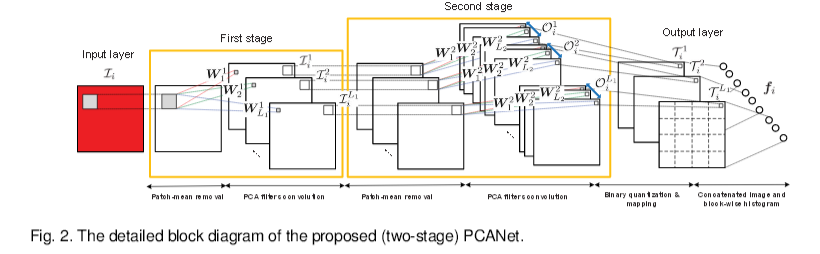
\includegraphics[scale=1.7,width=14cm]{pcanetstructure.png}
\end{center}
   \caption{The Architecture of PCANet}
\label{Fig: PCA Architecture}
\end{figure*}

%\begin{figure}[t] \label{Fig: PCA Architecture}
%\vspace{-15pt} \centering
%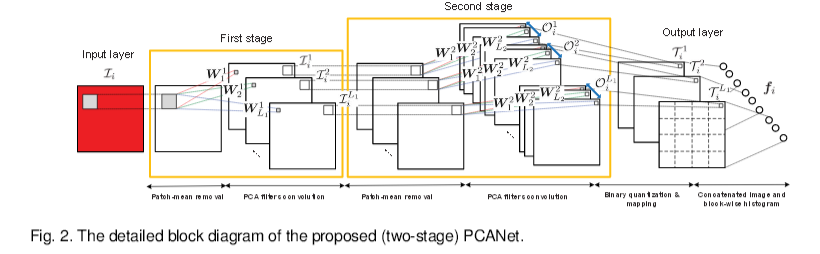
\includegraphics[scale=1.7,width=14cm]{pcanetstructure.png}
%\vspace{-20pt}\caption{The Architecture of PCANet}
%\end{figure}

\section{Models} 
Suppose that we are given $N$ input training images $\{\mathcal{I}_i\}_{i=1}^N $ of size $m \times n$, and assume that the patch size is $k_1 \times k_2$ at all stages in PCANet. The architecture of PCANet is shown in Figure \ref{Fig: PCA Architecture}. 

\subsection{The first stage of PCA Network (PCANet)}
Around each pixel, we take a $k_1 \times k_2$ patch, and we collect all (overlapping) patches of the $i$th image; i.e., $\b{x}_{i,1},...,\b{x}_{i,mn} \in \mathbb{R}^{k_1\times k_2}$. We then subtract mean from each patch and obtain $\bb{X} = [\bb{x}_{i,1},...,\bb{x}_{i,mn}] $. By constructing the same matrix for all input images and putting them together, we get
\begin{eqnarray}
	\b{X} = [\bb{X}_1,...,\bb{X}_N] \in \mathbb{R}^{k_1k_2\times Nmn}
\end{eqnarray}
In layer $1$, we can obtain the first $L_1$ PCA filters by minimizing the reconstruction error,i.e.
\begin{eqnarray}
	\b{\hat{V}} = \arg\min_{\b{V}\in \mathbb{R}^{k_1K_2\times L_1}} ||\b{X}-\b{VV}^T\b{X}||^2_F  \hspace{0.3cm} \textrm{s.t.} \hspace{0.2cm} \b{V}^T\b{V} = \b{I}
\end{eqnarray}
The solution is known as the $L_1$ principal vectors of $\b{XX}^T$. Then we can obtain the PCA filters by reshaping column $l$ of $\b{\hat{V}}$ to a matrix $\b{W}_l^1$ of dimension $k_1\times k_2$, for $l=1,...,L_1$. The $l$th filter output of the first stage is
\begin{eqnarray}
	\mathcal{I}_i^l =  \mathcal{I} * \b{W}_l^1
\end{eqnarray}
where $*$ denotes the 2D convolution. Therefore, the number of output of first stage is $L_1$, but the size of each output depends on the strides and number of zero paddings.



\subsection{The second stage of PCA Network (PCANet)}
Almost repeating the same process as the first stage. We can collect all the overlapping patches $\mathcal{I}_i^l$ from the first stage, and form $\bb{Y}^l = [\bb{y}_{i,l,1},...,\bb{y}_{i,l,mn}]  \in \mathbb{R}^{k_1K_2\times mn}$, where $\bb{y}_{i,l,j}$ is the $j$th mean-removed patch in $\mathcal{I}_i^l$. We further define $\b{Y}^l = [\bb{Y}_1^l,...,\bb{Y}_N^l]$ for the matrix collecting all the mean-removed patches of the $l$th filter, and concatenate $\b{Y}^l$ for all the filter outputs as 
\begin{eqnarray}
	\b{Y} = [\b{Y}^1,...,\b{Y}^{L_1}] \in \mathbb{R}^{k_1k_2\times L_1Nmn}
\end{eqnarray} 
The PCA filters of second stage are the eigenvectors of matrix $\b{YY}^T$. The number of outputs of the second stage is $L_1L_2$. 

\subsection{Output Stage} \label{subsection: Output Stage}
For each of the $L_1$ input images $\mathcal{I}_i^l$ for the second stage, it has $L_2$ real-valued outputs $ \{\mathcal{I}_i^l * \b{W}_l^2 \}$ from the second stage. We binarize the outputs and get $\{H(\mathcal{I}_i^l * \b{W}_l^2) \}$, where $H(x)=1$, if $x>0$ and $H(x)=0$ otherwise. Then we convert the $L_2$ outputs into a single integer-valued ``image":
\begin{eqnarray*}
	\mathcal{T}_i^l=\sum_{i=1}^{L_2} H(\mathcal{I}_i^l * \b{W}_l^2)
\end{eqnarray*} 
For each of the $L_1$ images, we partition it into $B$ blocks. Then we compute the histogram (with 32 bins, in \cite{chan2015pcanet}, they use $2^{L_2}$ bins) of the decimal values in each block, and concatenate all the B histograms into one vector. Thus the output vector has dimension $32 \times L_1 \times B$, if there is no overlap between the blocks. In \cite{chan2015pcanet}, this dimension is $2^{L_2} \times L_1 \times B$.

\section{Experiments on CIFAR10}
\subsection{CIFAR10 dataset}
For this dataset, we random select $5000$ images from training data as the validation data, and the rest $45000$ images are used as training data. We do not change the test data, which contains $10000$ images. 

\subsection{Training details}
We evaluate the PCANet and CNNs in CIFAR10 task, and compare the results with the state of the art and the baselines in \cite{chan2015pcanet}. The code is released at \url{https://github.com/tonyzhang1231/PCANet-CNN-torch}. Unfortunately, we haven't developed the GPU mode for this program, and only CPU mode is available at this moment.

For this task, the patch size of PCANet is fixed to $7 \times 7$, the stride is $1$ in both height and width direction, and no zero padding is imposed. The number of PCANet stages is $2$, and each stage has $8$ filters ($L_1=L_2=8$). In the output stage, the block size of histogram is $8 \times 6$, and the block overlap ratio is $0.5$. The PCA filters in stage 1 are displayed in Figure \ref{Fig: filters} (top).

For the fully connected networks applied to the PCA features. The filters are randomly initialized. The batch size is $64$. The learning rate is initialized at $0.001$, and it will decay with a factor of $0.9$ every $5$ epochs. The momentum is $0.9$. The max number of epochs is $100$.

For the CNN1, there are 2 convolutional layers, followed by 2 linear layers and a softmax layer. The first convolutional layer has 8 filters and the second has 16 filters, each of them is followed by a RELU and max pooling layer. The first linear layer has dimension $400 \times 120$ and the second has dimension $120 \times 10$. The loss function is cross entropy. The patch size is $5 \times 5$, The batchSize is $64$. The learning rate is initialized at $0.001$, and it will decay with a factor of $0.9$ every $5$ epochs. The momentum is $0.9$. The max number of epochs is $100$. The convolutional filters in the first layer are shown in Figure \ref{Fig: filters} (bottom).

For CNN2, there are 3 convolutional layers, followed by 3 linear layers and a softmax layer. The first convolutional layer has 32 filters and the second has 64 filters, each of them is followed by a RELU and max pooling layer. The third convolutional layer is a $1\times 1$ convolutional layer. The first linear layer has dimension $400 \times 1024$, the second has dimension $1024 \times 128$ and the third has dimension $128 \times 10$, each is preceded with a dropout layer with $p=0.5$ and a RELU layer. The loss function is cross entropy. The patch size is $5 \times 5$, The batchSize is $64$. The learning rate is initialized at $0.001$, and it will decay with a factor of $0.9$ every $5$ epochs. The momentum is $0.9$. The max number of epochs is $100$. 


\begin{figure*}
	\begin{center}
		
\includegraphics[scale=1.7,width=15cm]{PCA_filters.png}
		
\includegraphics[scale=1.7,width=15cm]{CNN_filters.png}
	\end{center}
	\caption{The PCA filters (top) and CNN filters (bottom)}\label{Fig: filters}
\end{figure*}

%\subsection{Object Recognition on CIFAR10}
For PCANet, we do not conduct additional preprocessing because the preprocessing is already included in the PCANet training procedure. For CNN, we normalize each channel by subtracting the mean from each channel and divide it by its standard deviation. 

All the programs are executed on a single CPU.

\subsection{Results}
Figure \ref{Fig: filters} shows the filters extracted by PCANet (top) and CNN-1 (bottom). From the filters we can see that the PCANet does not capture good features of CIFAR10 dataset. However, the CNN filters are much better.

Table \ref{Table: tbl1} shows the test accuacy and training time of PCANet and CNNs on a single CPU. Indeed, the training time claimed in \cite{chan2015pcanet} is half hour, but the device is not mentioned. 

\begin{table}[h]
	\begin{center}
		\begin{tabular}{|c|c|c|}
		\hline
		Model & test accuracy & training time \\
		\hline
		\hline
		PCANet + Linear & $59.06$ & $8$ hours\\
		\hline
		CNN-1 & $65.02$ &$0.75$ hour\\ 	
		\hline
		CNN-2 & $70.82$ & $1.5$ hours\\ 	
		\hline
		PCANet in \cite{chan2015pcanet} & $77.14$ & -\\
			\hline
		\end{tabular}
		\caption{Test accuacy and training time of PCANet and CNNs}
		\label{Table: tbl1}
	\end{center}
\end{table}

\subsection{Webpage}
We develop a webpage as a demo of CNN. Figure \ref{Fig: webpage} shows the webpage, which takes a url as input and return the prediction. The website of this page is http://www.ironmon.net:3000.

\begin{figure*}
	\begin{center}
		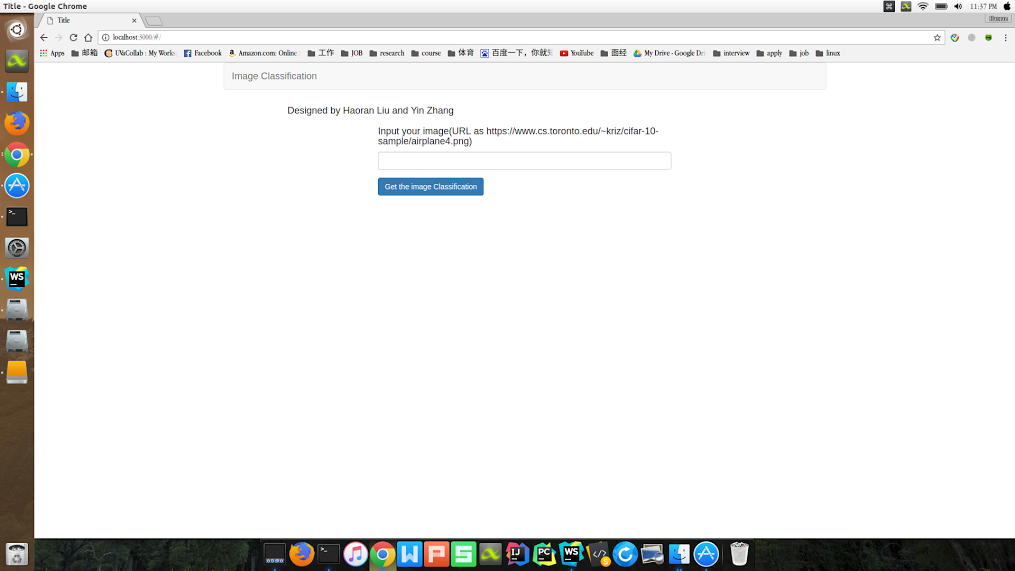
\includegraphics[scale=1.7,width=18cm]{webpage1.png}
		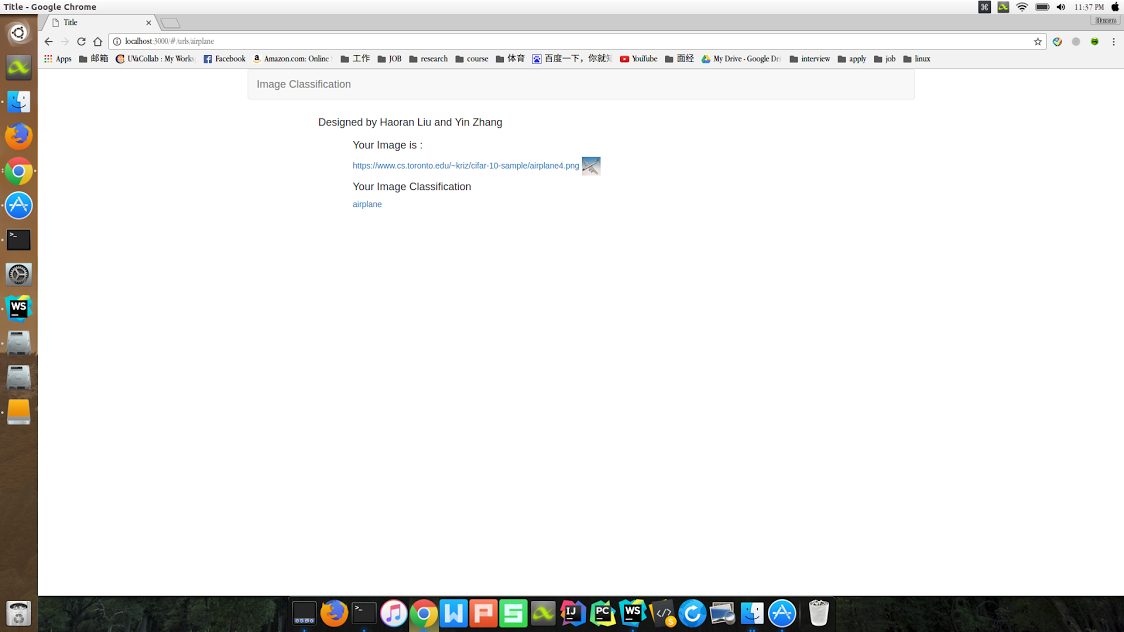
\includegraphics[scale=1.7,width=18cm]{webpage2.png}
	\end{center}
	\caption{}\label{Fig: webpage}
\end{figure*}


\section{Discussion}
In \cite{chan2015pcanet}, the output of the PCANet is $2^{L_2}L_1B$. If $L_1=L_2=8$ and $B=48$, the length of output is $98304$, which is much larger than the original image, which is $3\times 32 \times 32=3072$. This will cause the memory problem, because the PCA features are estimated to be more than $20$ gigabytes, and are not able to be fit in the memory. So in our work, we reduce the dimension of output vector to $3840$ by setting the number of bins to $32$ in section \ref{subsection: Output Stage}. This may explain the decrease in the performance compared with the result in \cite{chan2015pcanet}. 

The training time of PCA filter took around $3$ hours and the PCA features took another $3$ hours. The FC net took $2$ hours to go through $100$ epochs. Therefore, the total time is $8$ hours. However, the CNN-1 with $2$ layers only took less than $1$ hour to achieve a higher accuracy of $65.02\%$ and the CNN-2 only took $1.5$ hour to achieve a even higher accuracy of $70.82\%$.

We tried $500$ epochs for both the CNNs and PCANet, but the validation results do not change much after $50$ epochs, with the minimal learning rate $0.00001$. The validation accuracy of PCANet and CNNs are shown in Figure \ref{Fig: validation result}. As we can see the convergence of PCANet is faster than the CNNs. This is primarily because the PCANet already learned a good initial representation for the images, so the linear layers can converge in fewer iterations. The training accuracy approaches to $1$ as the number of epochs increases, although not presented here. 

Hence, we did not see too many advantages of the PCANet.

\begin{figure*}
	\begin{center}
		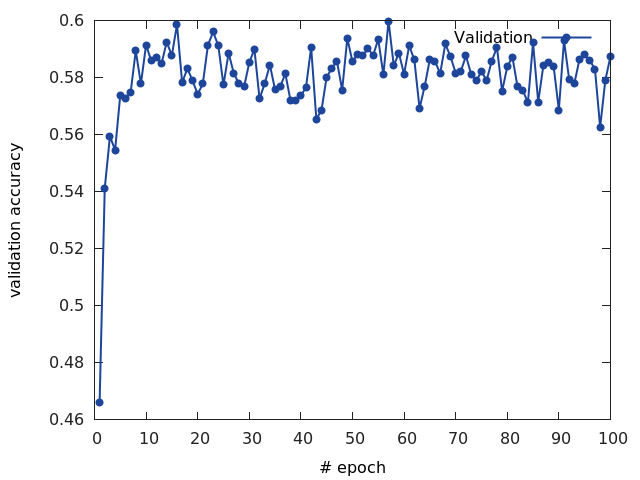
\includegraphics[scale=1.7,width=10cm]{PCANet_val_list.png} 
		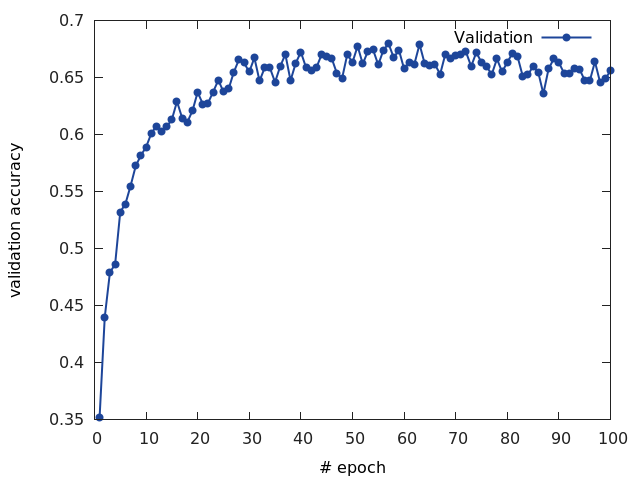
\includegraphics[scale=1.7,width=10cm]{CNN_val_list.png}
		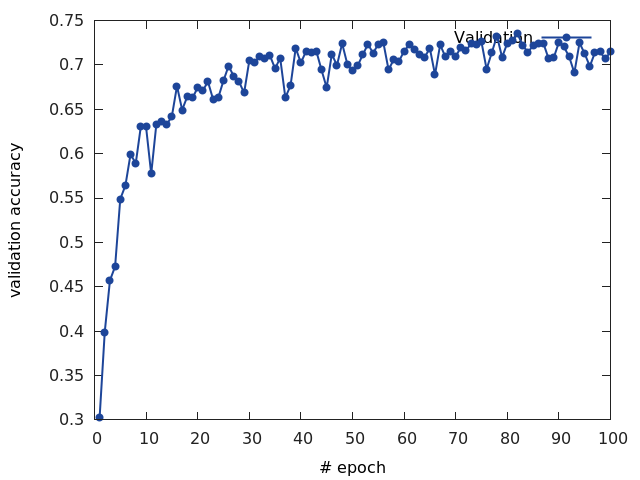
\includegraphics[scale=1.7,width=10cm]{DCNN_val_list.png}
	\end{center}
	\caption{The validation results (top) for PCANet, CNN-1 (middle) and CNN-2 (bottom)}\label{Fig: validation result}
\end{figure*}



\section{Future work}
To develop a nn.Module class for PCANet, which inherit the basic nn.Module class. Then it can be integrated into a larger network. The problem we can see so far is that the PCANet can not be placed in the middle of the network. Since if the input of the PCA layers change, we need to retrain the PCA filters, which is super computationally expensive.


{\small
\bibliographystyle{ieee}
\bibliography{mybib}
}

\end{document}
